\documentclass[11pt,a4paper]{scrartcl}
\usepackage[ngerman]{babel}
\usepackage[utf8]{inputenc}
\usepackage[T1]{fontenc}
\usepackage{graphicx}
\usepackage{float}
\usepackage{fullpage}
\usepackage{amssymb}
\usepackage{amsmath}
\usepackage[nounderscore]{syntax}
\usepackage{url}                % URLs
\usepackage{tikz}               % for the grey border on the title page
\usepackage{ziffer}				% to use commas as decimal separators in math mode
\usepackage{pdflscape}
\usepackage{multirow}
\usepackage{booktabs}
\usepackage{longtable, mdwtab}
\usepackage[absolute,overlay]{textpos}

\usepackage[a4paper,left=40mm,right=30mm,top=20mm,bottom=20mm,includeheadfoot]{geometry}
\newcommand{\changefont}[3]{\fontfamily{#1} \fontseries{#2} \fontshape{#3} \selectfont}
\parindent 0pt
\usepackage[raiselinks=true,
						bookmarks=true,
						bookmarksopenlevel=1,
						bookmarksopen=true,
						bookmarksnumbered=true,
						hyperindex=true,
						plainpages=false,
						pdfpagelabels=true,
						pdfborder={0 0 0.5},
						colorlinks=false,
						linkbordercolor={0 0.61 0.50},
						citebordercolor={0 0.61 0.50}]{hyperref}  %{0.57 0.74 0.57}

\author{PSE-Projekt 4 Team 2}
\title{Entwurfsdokument zu Worthwhile}

\setcounter{tocdepth}{1} % make TOC fit on one page

\hyphenation{Worth-while}

\newcommand{\reqtype}{}
\newenvironment{reqlist}[1]{\begin{description} \renewcommand{\reqtype}{#1}}{\end{description}}
\newcommand{\req}[3]{\item[\textbf{/\reqtype{}#1/}] #2 \\ #3}
\newcommand{\see}[1]{#1}
\renewcommand{\int}{\texttt{Integer}}
\newcommand{\bool}{\texttt{Boolean}}

\newcommand{\testspec}[4]{
		\begin{description}
			\item[Testziel] #1
			\item[Vorbedingungen] #2
			\item[Beschreibung] #3
			\item[Ergebnis] #4
		\end{description}}

\newcommand{\method}[1]{
			\item[\texttt{\textbf{#1}}]
            }
\newcommand{\attr}[1]{\item[\texttt{\textbf{#1}}]}
\newcommand{\type}[1]{\texttt{#1}}
\newcommand{\literal}[1]{\item[\texttt{#1}]}
\newcommand{\mlmethod}[1]{\method{\parbox{\textwidth}{#1}}}
\newenvironment{rcases}{%
  \left.\renewcommand*\lbrace.%
  \begin{cases}}%
{\end{cases}\right\rbrace}
\graphicspath{{images/}}

\begin{document}

%% titlepage.tex
%%

% coordinates for the bg shape on the titlepage
\newcommand{\diameter}{20}
\newcommand{\xone}{-30}
\newcommand{\xtwo}{150}
\newcommand{\yone}{15}
\newcommand{\ytwo}{-265}

\begin{titlepage}
% bg shape
\begin{tikzpicture}[overlay]
\draw[color=gray]
 		 (\xone mm, \yone mm)
  -- (\xtwo mm, \yone mm)
 arc (90:0:\diameter pt)
  -- (\xtwo mm + \diameter pt , \ytwo mm)
	-- (\xone mm + \diameter pt , \ytwo mm)
 arc (270:180:\diameter pt)
	-- (\xone mm, \yone mm);
\end{tikzpicture}

	\begin{textblock}{10}[0,0](1.7,1)
		
\includegraphics[width=.3\textwidth]{images/kit_logo_de_4c_positiv.pdf}
	\end{textblock}
	\changefont{phv}{m}{n}	% helvetica	
	\begin{center}
		\fontsize{45}{50}\selectfont
        \vfill
        \textsc{Worthwhile} \\
        \textsc{Pflichtenheft}
        \vfill
		\LARGE
		PSE WS 11/12
  \vfill
 \newpage
 
 \null
 \vfill
 
 Praxis der Softwareentwicklung -- WS 2011/2010 \\
  Automatisches Prüfen der Korrektheit von Programmen \\
  Projekt 4 -- Gruppe 2 \\
  \medskip
  \vspace{2cm}
  \Large
  \begin{tabular}{|l|l|}
    \hline
    Leon Handreke & 123456 \\
    \hline
    Chris Hiatt & 1610922 \\
    \hline
    Stefan Orf & 123456 \\
    \hline
    Joachim Priesner & 1579308 \\
    \hline
    Fabian Ruch & 123456 \\
    \hline
    Matthias Wagner & 1579342 \\
    \hline
  \end{tabular}
  \vspace{2cm} \\
  \today \\
	Revision 0
	\end{center}
	
  \vfill

\end{titlepage}


\tableofcontents
\clearpage

\section{Sprachdefinition}

\subsection{Trennung von Befehlen}

Die Trennung aufeinanderfolgender Befehle wird dadurch erreicht, dass in jeder Zeile höchstens ein Befehl stehen darf. Dies dient der Übersichtlichkeit, da hiermit Befehlstrenner wie das Semikolon unnötig werden.

\subsection{Operatorreihenfolge}

Die folgende Tabelle gibt die Reihenfolge an, in der Operatoren ausgewertet werden. Dabei werden die Operatoren mit höchster Priorität zuerst ausgewertet.

Operatoren mit gleicher Priorität werden von links nach rechts ausgewertet. Durch Klammersetzung kann die Auswertungsreihenfolge beeinflusst werden.

\begin{figure}[H]
\begin{tabular}{|l|l|}
\hline
\textbf{Priorität} & \textbf{Operatoren} \\
\hline
8 & \texttt{{[}\,{]}} \\
\hline
7 & $\neg, -, +$ (unäre Operatoren)\\
\hline
6 & $\cdot, \div, \%$\\
\hline
5 & $+, -$\\
\hline
4 & $<, \leq, \geq, >$\\
\hline
3 & $=$\\
\hline
2 & $\wedge$ \\
\hline
1 & $\vee$ \\
\hline
\end{tabular}
\end{figure}

\subsection{Formale Definition der Grammatik}

Ein Worthwhile-Programm besteht aus genau einem Element des Typs \textit{program}.

\setlength{\grammarindent}{12em} % increase separation between LHS/RH

\begin{grammar}

<program> ::= (<funcdecl> | <statement> | <axiom>)* 

<funcdecl> ::= `function' <type> <name> (<parameter>*) \\ (<requires> | <ensures>)* \\ <block>

<statement> ::= <vardecl> | <assign> | <block> | <annotation> | <funccall> | <conditional> | <loop> | <return>

<axiom> ::= `_axiom' (<expr> | <quantifiedexpr>)

<block> ::= `{' <statement>* `}'

<vardecl> ::= <parameter> `:=' <expr>

<assign> ::= <varref> `:=' <expr>

<varref> ::= <name> (`[' <expr> `]' )?

<annotation> ::= (`_assert' | `_assume') (<expr> | <quantifiedexpr>)

<funccall> ::= <name> `(' (<expr> (`,' <expr>)* )? `)'

<conditional> ::= `if' <expr> \\ <block>  \\ (`else' \\ <block>)?

<loop> ::= `while' <expr> \\ <invariant> \\ <block>

<invariant> ::= `_invariant' (<expr> | <quantifiedexpr>)

<return> ::= `return' <expr>

% TODO mark math symbols as tokens
<quantifiedexpr> ::= ($\forall$ | $\exists$ ) <type> <name> (`,' <expr>) (<quantifiedexpr> | `:' <expr>)

<expr> ::= <prefixop> <expr> | <expr> <binop> <expr> | <expr> <postfixop> | `(' <expr> `)' | <literal> | <varref> | <funccall>

<literal> ::= `false' | `true' | <integer>

<type> ::= <primitivetype> | <arraytype>

<primitivetype> ::= `Integer' | `Boolean'

<arraytype> ::= <primitivetype> `[' <expr> `]'

<parameter> ::= <type> <name>

<binop> ::= $\vee$ | $\wedge$ | $\textless$ | $\leq$ | $=$ | $\geq$ | $>$ | $+$ | $-$ | $\cdot$ | $/$

<prefixop> ::= $-$ | $+$ | $\neg$

<postfixop> ::= `[' <expr> `]'

<name> ::=  [`A--Za--z'][`A--Za--z0--9']*

\end{grammar}

\subsection{Reservierte Schlüsselwörter}

Folgende Schlüsselwörter sind für die Verwendung innerhalb der Sprache reserviert und dürfen daher nicht als Bezeichner für Variablen oder Funktionen verwendet werden:

\begin{itemize}
	\item \texttt{function}
	\item \texttt{Integer}
	\item \texttt{Boolean}
	\item \texttt{false}
	\item \texttt{true}	
	\item \texttt{\_axiom}
	\item \texttt{\_assert}
	\item \texttt{\_assume}
	\item \texttt{\_requires}
	\item \texttt{\_ensures}
	\item \texttt{if}
	\item \texttt{else}	
	\item \texttt{while}		
	\item \texttt{return}	
\end{itemize}

\subsection{Alternative Darstellungsweisen für mathematische Symbole}

Einige mathematische Symbole sind auf Tastaturen nicht verfügbar. Daher sind folgende textuelle Alternativen vorgesehen, um die Sprache auch ohne die Hilfe einer IDE editieren zu können:

\begin{figure}[H]
\begin{tabular}{|l|l|}
\hline
\textbf{Symbol} & \textbf{Alternative} \\
\hline
$\forall$ & \texttt{forall} \\
\hline
$\exists$ & \texttt{exists} \\
\hline
$\cdot$ & \texttt{*} \\
\hline
$\neg$ & \texttt{!} \\
\hline
$\vee$ & \texttt{\textbar\textbar} \\
\hline
$\wedge$ & \texttt{\&\&} \\
\hline
$\leq$ & \texttt{<=} \\
\hline
$\geq$ & \texttt{>=} \\
\hline
\end{tabular}
\end{figure}

\subsection{Typsystem}

Bedingt durch die kleine Anzahl möglicher Variablentypen ist das Typsystem nicht sehr komplex.

Jedes Sprachelement, das einen Wert zurückliefert, besitzt einen Rückgabetyp, kurz Typ des Sprachelements. Ein Sprachelement kann Kindelemente besitzen, deren Typ Einschränkungen unterliegen kann -- beispielsweise kann der Operator $+$ nur auf Operanden vom Typ \int{} angewendet werden.

In folgender Tabelle bedeutet die Notation $\rightarrow x$, dass der Typ des Sprachelements gleich dem Typ von $x$ ist.

\begin{landscape}

\enlargethispage{2cm}

\begin{figure}[H]
\begin{tabular}{lllp{11cm}}
\toprule
\textbf{Kategorie} & \textbf{Sprachelement} & \textbf{Typ} & \textbf{Einschränkungen} \\
\midrule
\multirow{4}{*}{Typdeklaration} & \int & \int & \\
\cmidrule{2-4}
& \bool & \bool & \\
\cmidrule{2-4}
& \multirow{2}{*}{$x$\texttt{[$N$]}} & \multirow{2}{*}{$\rightarrow x$} & $x \in \{$ \int{}, \bool{}$\}$ \\
& & & $N$ muss vom Typ \int{} sein \\
\midrule
Variablendeklaration & $type$ $name$ := $value$ & $\rightarrow type$ & Die Typen von $type$ und $value$ müssen gleich sein. \\
\midrule
\multirow{2}{*}{Variablenverweis} & $varref$ & $\rightarrow type$ & $type$ ist der in der Deklaration festgelegte Typ der Variablen. \\
\cmidrule{2-4}
& $varref$\texttt{[$index$]} & $\rightarrow varref$ & $index$ muss vom Typ \int{} sein. \\
\midrule
Variablenzuweisung & $varref$ := $value$ & $\rightarrow varref$ & Die Typen von $varref$ und $value$ müssen gleich sein. \\
\midrule
\multirow{6}{*}{Ausdrücke} & $x + y, x - y, x \cdot y, x \mathop{/} y, x \mathop{\%} y$ & \int & $x$ und $y$ müssen beide vom Typ \int{} sein. \\
\cmidrule{2-4}
& $a \wedge b, a \vee b$ & \bool & $a$ und $b$ müssen beide vom Typ \bool{} sein. \\
\cmidrule{2-4}
& $ -x, +x$ & \int & $x$ muss vom Typ \int{} sein. \\
\cmidrule{2-4}
& $\neg a$ & \bool & $a$ muss vom Typ \bool{} sein. \\
\cmidrule{2-4}
& \multirow{2}{*}{$x = y$} & \multirow{2}{*}{\bool} & $x$ und $y$ müssen beide vom gleichen Typ sein. \\
& & & $x$ und $y$ müssen vom Typ \int{} oder \bool{} sein. \\
\cmidrule{2-4}
& $x \leq y, x < y, x > y, x \geq y$ & \bool & $x$ und $y$ müssen beide vom Typ \int{} sein. \\
\midrule
Funktionsdeklaration & \texttt{function} $type$ $name$ ($params$) & $\rightarrow type$ & \\
\midrule
Funktionsverweis & $funcref$ & $\rightarrow type$ & $type$ ist der in der Deklaration festgelegte Rückgabetyp der Funktion. \\
\midrule
Funktionsaufruf & $funcref(params)$ & $\rightarrow funcref$ & Die Parameter $params$ müssen in Anzahl und jeweiligem Typ den deklarierten Parametern entsprechen. \\
\midrule
Rückgabewert & \texttt{return} $value$ & $-$ & Der Typ von $value$ muss gleich dem Rückgabetyp der umschließenden Funktion sein. \\
\bottomrule
\end{tabular}
\end{figure}
\end{landscape}

%\section{Grundlegende Entwurfsentscheidungen}
%
%\subsection{Polymorphic Dispatch}
%

\section{Abstract-""Syntax-""Tree (AST)}

\begin{landscape}
\begin{figure}%
    \vspace{-2cm}%
    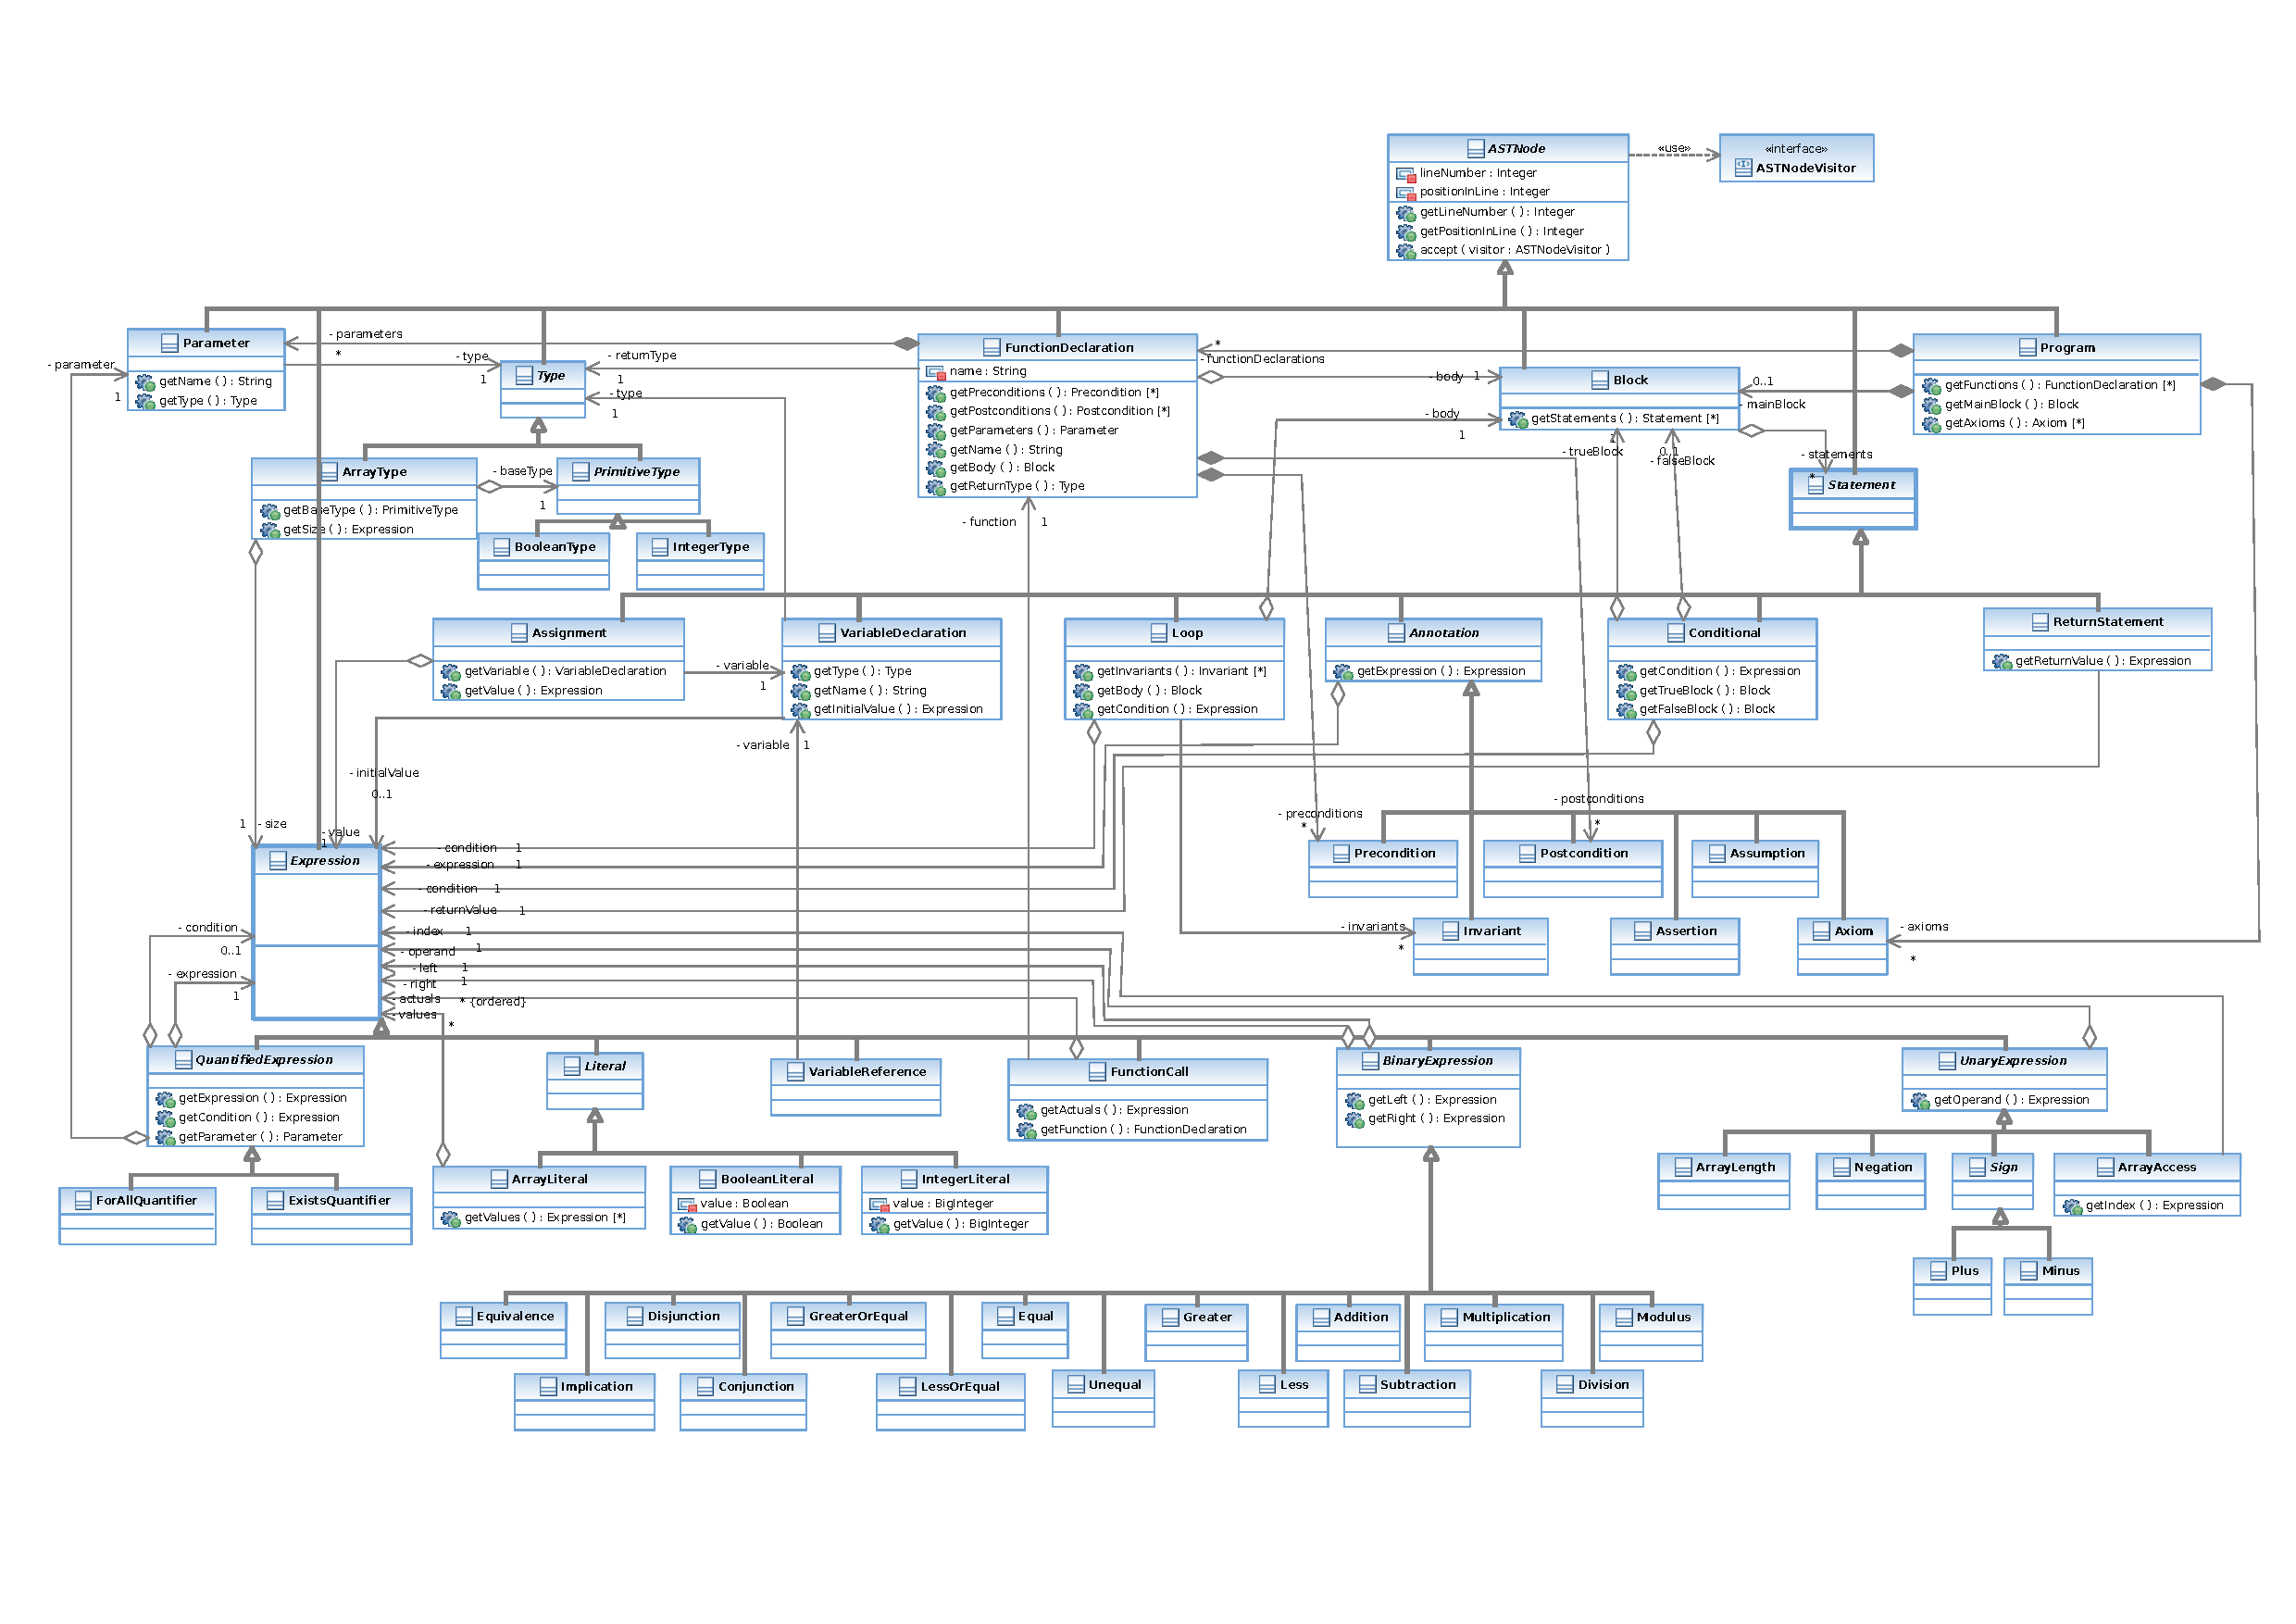
\includegraphics[height=\textheight]{diagrams/ast_component.pdf}

    \caption{Klassendiagramm des Abstract-""Syntax-""Trees mit den
    \type{Program}-""Bestandteilen \type{Statement} und
    \type{Expression} sowie der "`Besucher"'-""Klasse
    AST"-Node"-Visitor}

    \label{ast_diag}
\end{figure}%
\end{landscape}

\section{Parser}

Der Parser bietet die Funktionalität, einen Abstract-""Syntax-""Tree~(AST) aus einer in der WHILE-""Sprache verfassten Programmspezifikation zu generieren und dabei erkannte Syntaxfehler über seine Schnittstelle zugänglich zu machen.

\subsection{Klassenentwurf}

\subsubsection{class Parser}

Die Klasse Parser dient als Schnittstelle zum externen Parser und bündelt komplexe Vorgänge in einzelnen Methodenaufrufen. Hier kommt das Entwurfsmuster "`Fassade"' zur Anwendung.

\begin{description}
	\method{public Parser(source : String)}
	\method{public Parser(source : Readable)}
		Der Konstruktor der Klasse kann wahlweise mit einem String-""Parameter, welcher das zu parsende Programm enthält, oder einem \texttt{Readable}-Objekt, das beliebige Programmquellen zulässt, aufgerufen werden.

	\method{public getSyntaxErrors() : INode[*]}
		Diese Methode liefert eine Liste der Syntaxfehler, die beim Parsen erkannt wurden, zurück.

	\method{public getRootASTElement() : ASTNode}
		Hiermit wird das Wurzelelement des aus dem geparsten Programm generierten ASTs zurückgegeben.

	\method{public hasSyntaxErrors() : Boolean}
		Der Rückgabewert dieser Methode gibt an, ob während des Parsens Syntaxfehler aufgetreten sind.
\end{description}

\subsubsection{class Validator}

Diese Klasse wird ausschließlich innerhalb der Parser-Komponente zur semantischen Validierung des geparsten Programms benutzt.

\begin{description}
	\method{public checkTypesystemRules(node : ASTNode)}
    Überprüft den AST mit der übergebenen \texttt{ASTNode}-Wurzel auf Typfehler in Zuweisungen, Operandenangaben und Parameterübergaben.

	\method{public checkFunctionReferences(node : ASTNode)}
    Untersucht den übergebenen AST auf verwendete und nicht deklarierte Funktionen.

	\method{public checkVariableReferences(node : ASTNode)}
    Überprüft alle vorkommenden Variablen, ob sie vor ihrer Verwendung deklariert wurden.

	\method{public checkReturnStatements(node : ASTNode)}
    Überprüft, ob bei jedem möglichen Funktionsdurchlauf ein \texttt{return}-Statement erreicht wird.
\end{description}

\begin{figure}%

    \caption{Klassendiagramm der Komponente Parser}

    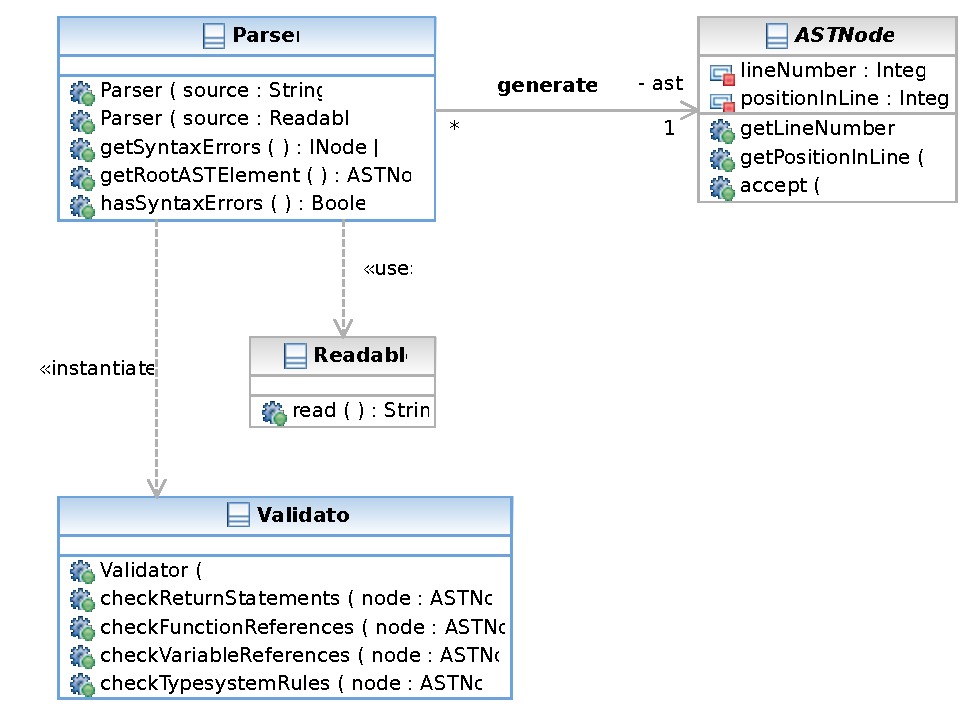
\includegraphics[width=\textwidth]{diagrams/parser_component.pdf}
\end{figure}%

% vim: spell spelllang=de:
\section{Interpreter}

Der Interpreter führt in der WHILE-""Sprache formulierte Programme aus und stellt eine Schnittstelle zum Debuggen von Programmen zur Laufzeit bereit. Des Weiteren überprüft er mit Hilfe des Evaluators zur Laufzeit die mittels Annotationen in den Programmtext eingebetteten Annotationen. Der Interpreter läuft in einem eigenen Thread und interagiert mit Hilfe von gemeinsam genutzten Datenstrukturen mit dem GUI-Thread.

\subsection{Eingabedaten}

\subsubsection{Programmspezifikation}

% copy-pasta von Beweiserschnittstelle oder ein neuer Abschnitt, der diesen Begriff einmal definiert?

\subsubsection{Klassenentwurf}

\subsubsection{class ExecutionContext}
Instanzen von \texttt{ExecutionContext} verwalten den Zustand eines Ausführungskontextes. Dazu gehören ein \texttt{ExpressionEvaluator}, ein \texttt{StatementExecutor} sowie eine \texttt{SymbolTable}, in der in diesem Kontext angelegte Symbole gespeichert werden.

%\begin{description}
%    \method{private SymbolTable symbolTable}
%    \method{private StatementExecutor statementExecutor}
%    \method{private ExpressionEvaluator expressionEvaluator}
%\end{description}

\begin{description}
<<<<<<< HEAD
    \method{public String getCurrentFunctionName()} % TODO should this really be a String?
    Gibt den Namen der in diesem Kontext ausgeführten Funktion zurück.
=======
    \method{public String getName()}
    Gibt einen Namen zurück, der diesem Kontext zugeordnet wurde. Normalerweise ist dies der Name der gerade ausgeführten Funktion.
>>>>>>> [ew] Add ReadableInterpreter, improve ExecutionContextStack

    \method{public SymbolTable getSymbolTable()}
    Gibt die aktuell gültige Symboltabelle zur Inspektion und Veränderung zrück.

    \method{protected void executeStatement(Statement statement)}
    Führt in diesem Kontext das angegebene Statement aus.

    \method{protected Object evaluateExpression(Expression expression)}
    Wertet in diesem Kontext die gegebene Expression aus und gibt das Ergebnis der Auswertung zurück.
\end{description}


\subsubsection{class ExecutionContextStack extends java.util.Stack<ExecutionContext>}

Instanzen von \texttt{ExecutionContextStack} verwalten eine Menge von "`gestapelten"' \texttt{ExecutionContext}-Objekten. Die Klasse \texttt{Interpreter} verwendet diesen Stack, um die für Funktionsaufrufe benötigten mehreren Instanzen von \texttt{ExecutionContext} einfach zu verwalten.

\subsubsection{class Interpreter}

Instanzen von \texttt{Interpreter} kontrollieren die Ausführung eines initial übergebenen Programms.

\begin{description}
    \method{public Interpreter(IParseResult parseResult)}
    Erzeugt eine Instanz, die das Programm, definiert durch die Parserausgabe \texttt{parseResult}, ausführen kann. Das Interface IParseResult wird vom Xtext Framework zur Verfügung gestellt und enthält neben dem AST Metainformationen wie beispielsweise die Positionen der Syntaxelemente im gelesenen Quelltext.

    \method{public void execute()}
    Startet die Ausführung des im Konstruktor übergebenen Programms in dieser Interpreter-""Instanz.

    \method{public void addDebugEventPolicy(AbstractDebugEventPolicy debugPolicy)}
    Fügt dem Interpreter eine Instanz einer Unterklasse von \texttt{AbstractDebugEventPolicy} hinzu und fügt sie der Menge der bei Ereignissen zu benachrichtigenden Objekte hinzu.

    \method{public void removeDebugEventPolicy(AbstractDebugEventPolicy debugPolicy)}
    Entfernt eine Instanz einer Unterklasse von \texttt{AbstractDebugEventPolicy} aus der Menge der bei Ereignissen zu benachrichtigenden Objekte.

    \method{public boolean addBreakpoint(int line)}
    Fügt einen Breakpoint in der gegebenen Zeile ein.

    \method{public boolean addBreakpoint(int line, \textbf{TODO} condition)} % Welche sprache?
    Fügt einen Breakpoint in der gegebenen Zeile ein, dessen Erreichen nur dann ein Ereignis auslöst, wenn die Aussage \texttt{condition} wahr ist.

    \method{public boolean clearBreakpoint(int line)}
    Entfernt den Breakpoint in der gegebenen Zeile.

    \method{public ExecutionContextStack getExecutionContextStack()} % TODO: in diesen Strukturen nur manche sachen public machen!
    Entfernt den Breakpoint in der gegebenen Zeile.

    %\method{public void executeStatement(Statement s)}
    %Führt das gegebene Statement aus und aktualisiert bei Bedarf die Symboltabelle.
\end{description}

\subsubsection{class ReadableInterpreter extends Interpreter}

\begin{description}
    \method{public ReadableInterpreter(Readable inputReadable)}
    Konstruiert eine neue \texttt{Interpreter}-""Instanz durch Lesen der Spezifikation des Programms in der WHILE-""Sprache aus dem übergebenen Readable-""Objekt.
\end{description}


\subsubsection{interface ExpressionEvaluator}
Die Aufgabe von \texttt{ExpressionEvaluator} Instanzen ist es, \texttt{Expression} Objekte aus dem AST auszuwerten.
\begin{description}
    \method{public Object eval(Expression expression)}
    Wertet die Expression \texttt{expression} aus und gibt das Ergebnis zurück.
\end{description}

\subsubsection{class InterpreterExpressionEvaluator implements ExpressionEvaluator}
Wertet Expressions aus, für die zur Auswertung Zugriff auf den \texttt{ExecutionContext} sowie den \texttt{Interpreter} nötig ist, beispielsweise um Funktionsaufrufe auszuwerten oder die Werte referenzierter Variablen aufzulösen.

\subsubsection{abstract class AbstractDebugEventPolicy}
Instanzen von Unterklassen von \texttt{AbstractDebugEventPolicy} behandeln Ereignisse, die bei der Ausführung des Programms auftreten. Die Methoden dieser Klasse werden dabei vom Interpreter synchron aufgerufen, was es dem Policy-Objekt erlaubt, die Ausführung anzuhalten oder zu verzögern. Dabei müssen nicht alle Methoden überschrieben werden -- eine Unterklasse von AbstractDebugEventPolicy kann auch nur auf eine Teilmenge der definierten Ereignisse reagieren.

\begin{description}
    \method{protected void statementExecuted()}
    Wird vom Interpreter nach jedem Ausführen eines Statements aufgerufen.
    \method{protected void expressionEvaluated()}
    Wird vom Interpreter nach jedem Auswerten einer Expression aufgerufen.
    \method{protected void executionStarted()}
    Wird vom Interpreter direkt nach dessen Start aufgerufen.
    \method{protected void executionTerminatedNormally()}
    Wird vom Interpreter nach ordnungsgemäßer Terminierung des Programms aufgerufen.
    \method{protected void executionTerminatedAbnormally()}
    Wird vom Interpreter nach einer fehlerbedingten Terminierung des Programms, ausgelöst beispielsweise durch einen Laufzeitfehler, aufgerufen.
    \method{protected void breakpointReached()}
    Wird vom Interpreter aufgerufen, nachdem ein Breakpoint erreicht (und gegebenenfalls die damit assoziierte Bedingung als wahr ausgewertet) wurde.
    \method{protected void assertionSucceeded()}
    Wird vom Interpreter nach jeder erfolgreichen Ausführung einer Zusicherungsinstruktion aufgerufen.
    \method{protected void assertionFailed()}
    Wird vom Interpreter nach jeder fehlgeschlagenen Ausführung einer Zusicherungsinstruktion aufgerufen.
\end{description}

\section{Beweiserschnittstelle}%

Die Beweiserschnittstelle lässt Worthwhile-""Programmspezifikationen
und -""Annotationen mit Kontext von einem Beweiser überprüfen
und liefert dem Aufrufer dessen Auswertung zurück. Die Auswertung
besteht aus einem Wahrheitswert, einem Modell und einer Liste von
Fehlerausgaben.%

\subsection{Eingabedaten}%

\subsubsection{Programmspezifikation}%

% TODO Datentyp des Abstract-Syntax-Tree

Die Programmspezifikation wird dem Abstract-Syntax-Tree~(AST), welcher
aus einem Worthwhile-Text erstellt wurde, entnommen. Sie setzt sich
zusammen aus dem WHILE-Programmtext und den Annotationen. Annotationen
sind entweder Axiome, Funktionsverträge, Schleifeninvarianten,
Zusicherungen oder Annahmen.%

Siehe \texttt{SpecificationChecker::checkProgram}%

\subsubsection{Annotationen mit Kontext}%

Der Beweiserschnittstelle wird ein AST übergeben, der genau einen
Annotationsausdruck enthält, also insbesondere kein WHILE-Programmtext
oder Annotationstyp. Zusätzlich kann ein Modell als Auswertungskontext
angegeben werden, das im Ausdruck freien Variablen eine Bedeutung
zuweist. Dieses Modell kann zum Beispiel einem Ausführungszustand
entsprechen, sodass Annotationsausdrücke auch für konkrete
Ausführungen (anstatt für alle wie bei
Programmspezifikationsprüfungen) geprüft werden können.%

Siehe \texttt{SpecificationChecker::checkAnnotation}%

\subsection{Formelerstellung im wp-Kalkül für den Beweiser Z3}%

Die Erstellung einer Formel aus einer Programmspezifikation im
wp-Kalkül ist eine Implementierung der Schnittstelle
\texttt{FormulaGenerator} und die Benutzung des Beweisers Z3 für
erstellte Formeln ist eine Implementierung der Schnittstelle
\texttt{ProverCaller}. Beide Implementierungen werden von Worthwhile
mitgeliefert.%

\subsubsection{Axiome}%

Die schließlich an den Beweiser übergebene Formel ist eine
Implikation, auf deren linken Seite die konjunktiv verknüpften Axiome
stehen. Wenn keine Axiome angegeben wurden, steht auf der linke Seite
der Implikation der Wahrheitswert \texttt{true}. Auf der rechten Seite
steht das zu beweisende Theorem, dass das Programm der Spezifikation
entspricht.%

Axiome sind im AST als \texttt{axiom}-Knoten codiert und die Kinder
sind syntaktische Elemente prädikatenlogische Formeln.%

\subsubsection{Funktionsverträge}%

Funktionen werden modular spezifiziert. Ihre Spezifikation besteht aus
den Annahmen, die ihre Parameter für Ergebniskorrektheit erfüllen müssen, und den
Zusicherungen, die sie bei gültigen Parametern für ihr Ergebnis
erfüllen. Annahmen werden Vorbedingungen genannt, Zusicherungen
Nachbedingungen und die Menge aller dieser Bedingungen Funktionsvertrag.%

Für den Funktionsprogrammtext werden die Vorbedingungen wie Axiome behandelt
und Nachbedingungen wie Zusicherungen für den Rückgabewert der
Funktion.%

Vorbedingungen werden im AST als \texttt{requires}-Knoten und
Nachbedingungen als \texttt{ensures}-Knoten codiert. Die Kinder beider
Knotentypen sind syntaktische Elemente prädikatenlogischer Formeln.%

Siehe \texttt{FP020}%

\subsubsection{Schleifeninvarianten}%

Schleifeninvarianten werden in der Formel an den Beweiser so
eingebettet, dass ihre Aussagen vor dem Schleifeneintritt, nach jedem
Durchlauf und nach dem Austritt gelten müssen. Nach jedem Durchlauf
heißt, dass die Erfülltheit der Schleifenbedingung und der Invariante
die Aussage der Invariante impliziert, und nach dem Austritt bedeutet
analog, dass die Erfülltheit der negierten Schleifenbedingung und der
Invariante wiederum die Aussage der Invariante impliziert.%

Schleifeninvarianten werden im AST als \texttt{invariant}-Knoten
codiert, deren Kinder syntaktische Elemente prädikatenlogischer
Formeln sind.%

Siehe \texttt{FP030}%

\subsubsection{Zusicherungen}%

Zusicherungen werden in der Formel an den Beweiser so eingebettet,
dass ihre Aussage bei jeder Programmausführung durch den
vorhergehenden Programmtext erfüllt sein muss.%

Zusicherungen werden im AST als \texttt{assert}-Knoten codiert, deren
Kinder syntaktische Elemente prädikatenlogischer Formeln sind.%

\subsubsection{Annahmen}%

Annahmen werden wie Axiome behandelt, sodass sie insbesondere nicht
wie Zusicherungen erfüllt sein müssen und vom Beweiser auch nicht auf Erfülltheit
geprüft werden.%

Annahmen werden im AST als \texttt{assume}-Knoten codiert,
deren Kinder syntaktische Elemente prädikatenlogischer Formeln sind.%

\subsubsection{Arrayzugriffe}%

Für Arrays werden implizit die drei Axiome (A1), (A2) und (A3)
vorausgesetzt. Außerdem wird jedem Arrayzugriff im Programmtext bei
der Formelerstellung die Zusicherung, dass der angegebene Feldindex
nicht negativ ist und nicht die Deklarationsgröße übersteigt, vorangestellt.%

\begin{description}%
    \item[A1] \begin{math}\forall i \in \mathbb{A}, e \in \mathbb{B} : \{\texttt{true}\} a[i] := e \{a[i] = e\}\end{math}%
    \item[A2] \begin{math}\forall i, j \in \mathbb{A}, e, f \in \mathbb{B} : \{i \neq j \wedge a[i] = e\} a[j] := f \{a[i] = e\}\end{math}%
    \item[A3] \begin{math}\forall a, b \in \mathbb{B}^\mathbb{A} : (\forall i, j \in \mathbb{A} : a[i] = b[j]) \Rightarrow a = b\end{math}%
\end{description}%

\subsubsection{Division}%

Ausdrücken, die eine Division durchführen, wird implizit die Zusicherung
vorangestellt, dass der Dividend ungleich Null ist. Damit wird erreicht, dass
die Möglichkeit eines Programmdurchlaufs, der eine Division durch Null enthält,
auch bei der Prüfung der Spezifikation erkannt und das spezifizierte Programm
nicht als korrekt eingestuft wird, obwohl nicht alle Programmaufrufe mit
definiertem Ergebnis terminieren.%

\subsubsection{Typsystem}%

Die in Worthwhile vorhandenen Datentypen \texttt{Integer} und
\texttt{Boolean} werden beide von dem Beweiser Z3 unterstützt. Die Typen verwendeter Sprachelemente
werden bei Parameterübergabe, Symbolreferenz und Symboldefinition
geprüft. Treten in einem dieser Fälle nicht übereinstimmende Typen auf, liefert Z3 einen
Fehler. Diese Fehler sind in der \texttt{ProverResult}-Rückgabe enthalten.%

\subsection{Kontext für einzelne Annotationen}%

% TODO Datentyp für Programmzustand und ausgewertete Annotationen

Die Bedeutungszuweisung für freie Variablen im Annotationsausdruck werden wie
Axiome behandelt.%

\subsection{Ausgabedaten}%

\subsubsection{Modell}%

Modelle verifizieren die Erfüllbarkeit von prädikatenlogischen
Formeln, indem sie freie Variablen auf genau ein Element ihrer Domäne
abbilden. Ein Modell, das die Beweiserschnittstelle liefert, besteht
ausschließlich aus Abbildungen, die hinreichend für eine
verifizierende Auswertung der geprüften Formel sind und sich auf im
geprüften Programmteil nicht initialisierte Variablen (z.~B.\
Parameter) beziehen.%

\subsubsection{Fehlerausgaben}%

\subsection{Klassenentwurf}%

\begin{itemize}%

    \item Zur Transformation einer Programmspezifikation werden für
    \texttt{WWAST} Besucherklassen für die einzelnen syntaktischen
    Elemente implementiert.%

    \item Die Besucher hängen von Strategieklassen ab, welche die
    Transformationsregeln und die Formelsprache austauschbar machen.%

    Siehe \texttt{Prover::ProgramTransformer::FormulaGenerator}%

    Siehe \texttt{Prover::TheoremProver::FormulaCompiler}%

    % TODO Spezifikation des unterstützten SMT-LIB-Standards

\end{itemize}%

\subsubsection{class Environment}%

Instanzen von \texttt{Environment} fassen einen Programmzustand
zusammen. Dazu gehören sowohl Wertbelegungen für Symbole als auch
erfüllte Annotationen.%

\subsubsection{class WWAST}%

Instanzen von \texttt{WWAST} codieren Programmtexte, welche der Syntax
von Worthwhile entsprechen.%

\subsubsection{class Prover::Formula}%

Formula beschreibt Instanzen, die prädikatenlogische Formeln als
Syntaxbaum \footnote{Die Syntax prädikatenlogischer Formeln ist
\url{http://formal.iti.kit.edu/teaching/pse/2011/Downloads/intro.pdf}
entnommen} zugänglich machen.%

\subsubsection{class Prover::SpecificationChecker}%


% TODO nicht öffentliche Attribute

\begin{description}%
    \method{private int timeout}%

    Zeit in Sekunden, nach der \texttt{check""Program} und
    \texttt{check""Annotation} zurückkehren müssen.%

    Siehe \texttt{setTimeout}.%

    \method{private Map<VariableRef,Literal> model}%

\end{description}%

% TODO öffentliche Methoden

\begin{description}%
    \method{public SpecificationChecker(ProverCaller prover, FormulaGenerator generator)}%

    \method{public bool checkProgram(WWAST program)}

    Prüft mit Hilfe eines Beweisers die Korrektheit des annotierten
    Programms \texttt{prg}. Es wird genau dann \texttt{true}
    zurückgeliefert, wenn \texttt{prg} für alle Ausführungen den
    Annotationen entspricht, und \texttt{false} sonst~(z.~B.\, wenn
    \texttt{timeout} überschritten wurde oder die Spezifikation für
    eine Ausführung nicht erfüllt wird).%

    Siehe \texttt{getModel}%

    Siehe \texttt{FP005}%

    \method{public bool checkAnnotation(WWAST annotation, Environment env)}

    Prüft mit Hilfe eines Beweisers die Erfülltheit der Annotation
    \texttt{ann}. Es wird genau dann \texttt{true} zurückgeliefert,
    wenn \texttt{ann} im Kontext \texttt{env} erfüllt ist, und
    \texttt{false} sonst~(z.~B.\, wenn \texttt{timeout} überschritten
    wurde).%

    Siehe \texttt{getModel}%

    Siehe \texttt{FP005}%

    \method{public Environment getModel()}

    Liefert für den vorhergehenden Aufruf von \texttt{check""Program}
    oder \texttt{check""Annotation} die Ausgabe des Beweisers und
    \texttt{null}, wenn zuvor weder ein Programm noch eine Annotation
    überprüft wurde oder keine Ausgabe verfügbar war.%

    \method{public void setTimeout(int seconds)}

    Setzt den Timeout für Aufrufe von \texttt{check""Program} und
    \texttt{check""Annotation} auf den Wert von \texttt{seconds}. Ist
    der angegebene Wert negativ, wird er als Null interpretiert.%

\end{description}%

\subsubsection{interface Prover::ProgramTransformer::FormulaGenerator}%

Implementierungen dieser Schnittstelle erstellen aus einem
Worthwhile-""Programmtext eine prädikatenlogische Formel. Diese Formel
soll nur dann beweisbar sein, wenn das Programm seine Spezifikation
erfüllt. Diese Korrektheit bezieht sich immer auf ein Kalkül, weshalb
Implementierungen dieser Schnittstelle meistens die Produktionsregeln
eines solchen formalen Systems kapseln.%

\begin{description}%
    \method{protected Formula transformProgram(WWAST root)} %

    Liefert die aus \texttt{root} transformierte \texttt{Formula}
    zurück. Die Semantik der Formel ist unbestimmt, falls der
    Programmtext kein semantisch korrektes Programm beschreibt, also
    nicht ausgeführt werden kann. Ansonsten ist die zurückgelieferte
    Formel nur dann beweisbar, wenn im angewendeten Kalkül das
    WHILE-""Programm für alle Ausführungen seinen Annotationen
    entspricht.%

    Parameter \texttt{root}: Wurzelsprachelement des zu
    transformierenden Worthwhile-""Programms, d.~h.\ sowohl der
    WHILE-""Programmtext als auch dessen Annotationen sind im
    Syntaxbaum enthalten.%

\end{description}%

\subsubsection{interface Prover::TheoremProver::ProverCaller}%

Implementierungen dieser Schnittstelle kapseln Aufrufe eines Beweisers
für gegebene prädikatenlogische Formeln. Das Ergebnis eines Aufrufs
besteht aus der Formelerfüllbarkeit, einem Modell zur Verifikation
derselben und einer Liste semantischer Fehler.%

\begin{description}%
    \method{protected ProverResult checkFormula(Formula formula)}%

    Aufruf des unterstützten Beweisers für die Überprüfung der
    prädikatenlogischen Formel \texttt{formula}. Es wird nur dann
    \texttt{true} in \texttt{ProverResult\#satisfiable}
    zurückgeliefert, wenn die Formel erfüllbar ist, und \texttt{false}
    sonst. Ist \texttt{ProverResult\#satisfiable} auf \texttt{true}
    gesetzt, muss \texttt{ProverResult\#model} mit einem
    entsprechenden Modell als Zeuge und \texttt{ProverResult\#errors}
    mit einer leeren Liste initialisiert sein.%

    Parameter \texttt{formula}: Wurzelsprachelement der zu prüfenden
    prädikatenlogischen Formel.%

\end{description}%

\subsubsection{abstract class Prover::TheoremProver::StdProver extends ProverCaller}%

Instanzen von dieser Abstraktion abgeleiteter Klassen rufen Beweiser
auf, denen die zu überprüfende Formel auf der Standardeingabe
übergeben wird. Spezialisierungen dieser Klasse implementieren die
Extrahierung des Beweiserergebnisses aus der Standardausgabe.%

\begin{description}%
    \method{protected StdProver(String path, FormulaCompiler compiler)}%

    Konfiguriert Instanzen so, dass der Beweiser \texttt{path} mit dem
    Formelkompilat von \texttt{compiler} für zu überprüfende
    prädikatenlogische Formeln aufgerufen wird.%

    Parameter \texttt{path}: Systempfad der ausführbaren Datei eines
    Beweisers.%

    Parameter \texttt{compiler}: Wird zur Generierung der
    Beweisereingabe aus einer angegebenen prädikatenlogischen Formel
    aufgerufen.%

    \method{override protected ProverResult checkFormula(Formula formula)}%

    Ruft den bei Objekterstellung angegebenen Beweiserpfad auf und
    füllt die Standardeingabe mit dem vom angegebenen Compiler aus
    \texttt{formula} erstellten Kompilat auf.
    \texttt{ProverResult\#satisfiable} wird auf \texttt{false}
    gesetzt, falls bei der Beweiserausführung ein Systemfehler
    aufgetreten ist, und sonst wird die Rückgabe von
    \texttt{getResult} zurückgeliefert, welche den Inhalt der
    Standardausgabe nach Beweiseraufruf erhalten hat.%

    \method{abstract protected ProverResult getResult(String output)}%

    Extrahiert aus \texttt{output} sowohl Ergebnis als auch Fehler
    eines Beweiseraufrufs und liefert diese Informationen in einer
    Instanz von \texttt{ProverResult} zurück. Kann der Inhalt von
    \texttt{output} nicht interpretiert werden, wird
    \texttt{ProverResult\#satisfiable} auf \texttt{false} gesetzt.%

    Parameter \texttt{output}: Textausgabe nach einem Beweiseraufruf.%

\end{description}%

\subsubsection{interface Prover::TheoremProver::FormulaCompiler}%

Implementierungen dieser Schnittstelle übersetzen eine
\texttt{Formula} in die Eingabesprache eines Beweisers, sodass dieser
mit der zurückgelieferten Zeichenkette die Erfüllbarkeit der
ursprünglichen Formel prüfen und seine Ausgabe in ein verifizierendes
Modell zurückübersetzt werden kann.%

\begin{description}%
    \method{protected String compileFormula(Formula formula)}%

    Liefert eine Übersetzung von \texttt{formula} in eine
    Beweisersprache, sodass das erfüllende Modell eines Beweisers, der
    diese Sprache interpretiert, genau auf ein erfüllendes Modell von
    \texttt{formula} abbilden lässt~(Bedeutungserhalt).%

    %\method{protected Formula uncompileFormula(String formula)}%

\end{description}%

\subsection{Interaktionsentwurf}%

\section{Grafische Benutzeroberfläche (GUI)}

Die GUI bietet eine grafische Schnittstelle zur Steuerung aller Komponenten von Worthwhile. Während wichtige Komponenten wie Interpreter und Beweiser auch ohne die GUI ausgeführt werden können, erleichtert eine grafische Oberfläche das Arbeiten mit ihnen ungemein.

Die GUI enthält alle Funktionen, die man von einer modernen integrierten Entwicklungsumgebung erwartet. Dazu gehört insbesondere ein Editor mit Syntaxhervorhebung, Code Folding und Markierung von Parserfehlern während der Eingabe. Weiterhin bietet sie Funktionen zum Ausführen des Interpreters und des Beweisers sowie einen Debugger.

Die GUI benutzt das Entwurfsmuster \textit{Model-View-Controller.} Dabei ist der AST das Modell, das von diversen Sichten (Views) wie dem Editor, der Parserfehler-Ansicht oder dem Projektexplorer angezeigt wird. Über GUI-Befehle werden Änderungen am Modell ausgelöst, sodass die GUI selbst hier als Controller fungiert.

Weitere eingesetzte Entwurfsmuster sind \textit{Strategy} etwa bei der Bereitstellung von AutoEdits und bei den Provider"-klassen (\texttt{Label"-Provider}, \texttt{Quickfix"-Provider}, \texttt{Outline"-Tree"-Provider} etc.) sowie \textit{Plugin}, da die Worthwhile-Komponente in die existierende Eclipse-Plattform über Plugins eingebunden wird. Diese Plugins implementieren Schnittstellen, die durch die Plattform vorgegeben sind.

\subsection{Klassenentwurf}

\subsubsection{class WorthwhileEditor}

Der Editor dient zur Bearbeitung von Dateien vom Typ Worthwhile-Programm (Dateiendung \texttt{.ww}). Für jede geöffnete Datei erstellt die GUI eine neue Instanz dieser Klasse.

\begin{description}
	\method{public IResource getResource()} Gibt die vom Editor bearbeitete Ressource zurück. In diesem Fall ist dies eine Datei, also eine Instanz einer Klasse, die \texttt{IFile} implementiert.
	\method{public bool isEditable()} Gibt zurück, ob die im Editor geöffnete Datei zum aktuellen Zeitpunkt verändert werden kann.
\end{description}

\subsubsection{class WorthwhileLabelProvider}

Der Label Provider dient dazu, einem Sprachelement eine Beschriftung und ein Symbol zuzuweisen. Wo in der GUI eine textuelle Repräsentation eines Sprachelements angezeigt werden muss (etwa in Tooltips oder bei der Codevervollständigung), wird auf den \texttt{LabelProvider} zurückgegriffen.

\begin{description}
	\method{public String getText(element : EObject)} Gibt den Beschriftungstext für das Sprachelement \texttt{element} zurück.
	\method{public String getImage(element : EObject)} Gibt den Dateinamen eines Symbols für das Sprachelement \texttt{element} zurück.
\end{description}

\subsubsection{class WorthwhileDescriptionLabelProvider}

In manchen Fällen müssen Beschriftungstexte und Symbole für Sprachelemente angezeigt werden, ohne dass die entsprechende Datei geöffnet ist. Ein Beispiel dafür ist die Fehlerübersicht, in der alle Parserfehler der Dateien eines Projekts angezeigt werden, auch wenn die Datei nicht in einem Editor geöffnet ist. Dazu wird in einem internen Cache der GUI für jedes Sprachelement einer Datei eine sogenannte Beschreibung (\texttt{IEObjectDescription}) abgelegt. Der \texttt{DescriptionLabelProvider} dient dazu, aus einer solchen Beschreibung einen Beschriftungstext und ein Symbol zu extrahieren.

\begin{description}
	\method{public String getText(description : IEObjectDescription)} Gibt den Beschriftungstext für das durch \texttt{description} beschriebene Sprachelement zurück.
	\method{public String getImage(description : IEObjectDescription)} Gibt den Dateinamen eines Symbols für das durch \texttt{description} beschriebene Sprachelement zurück.
\end{description}

\subsubsection{class WorthwhileQuickfixProvider}

Da durch den \texttt{Validator} nicht nur syntaktische, sondern auch semantische Fehler erkannt werden sowie durch den \texttt{SyntaxErrorMessageProvider} die Art eines Syntaxfehlers näher spezifiert werden kann, ist es möglich, für bestimmte Fehler und Warnungen eine Reihe von Korrekturvorschlägen anzubieten. Der Benutzer kann einen dieser Korrekturvorschläge zur automatischen Anwendung auswählen.

Die in dieser Klasse spezifizierten Korrekturfunktionen erhalten als Parameter jeweils eine Fehlerbeschreibung (\texttt{Issue}) sowie eine Referenz auf einen \texttt{Issue"-Resolution"-Acceptor}, der die Korrekturvorschläge entgegennimmt und an die GUI weiterleitet.

\begin{description}
	\mlmethod{public void addFunctionReturnType(issue : Issue, \\ acceptor : IssueResolutionAcceptor)} Bietet für eine Funktion mit nicht spezifiziertem Rückgabetyp das Hinzufügen eines Rückgabetyps an.
	%\method{TODO}
\end{description}

\subsubsection{class WorthwhileOutlineTreeProvider}

Für größere Programmdateien ist es eine Hilfe, die in einem Programm vorkommenden Elemente wie Funktions- und Variablendeklarationen auf einen Blick zu sehen. Die GUI bietet diese Möglichkeit, indem im \textit{Outline}-Fenster eine hierarchische Ansicht des Programmtextes angezeigt wird. Diese Ansicht wird durch den \texttt{OutlineTreeProvider} erstellt.

\begin{description}
	\method{public IOutlineNode createRoot(document : IXtextDocument)} Erstellt den Wurzelknoten der hierarchischen Ansicht aus dem Dokument \texttt{document}.
	\method{public void createChildren(parent : IOutlineNode, modelElement : EObject)} Erstellt die Kindknoten des gegebenen Knotens \texttt{parent} in der Outline-Ansicht, wobei der Knoten \texttt{parent} das Sprachelement \texttt{modelElement} repräsentiert.
\end{description}

\subsubsection{class WorthwhileProposalProvider}

Für die Code-Vervollständigung muss eine Reihe von Vorschlägen erstellt werden. Während sich die meisten direkt aus der Grammatik und den schon vorhandenen AST-Elementen ableiten lassen, kann es wünschenswert sein, eigene Vorschläge zu erstellen oder vorhandene anzupassen. Diese Aufgabe übernimmt der \texttt{ProposalProvider}.

\begin{description}
	\mlmethod{public void complete\_$\{$RegelName$\}$(model : EObject, ruleCall : RuleCall, context~:~ContentAssistContext, acceptor~:~ICompletionProposalAcceptor)} Übergibt eine Liste von Vervollständigungs-Vorschlägen an das \texttt{acceptor}-Objekt, das sie an die GUI weiterleitet. Dabei ist \texttt{RegelName} die Regel aus der Sprachdefinition, für die Vorschläge erstellt werden sollen. Wird beispielsweise an der aktuellen Stelle im Programm gemäß Sprachspezifikation eine Zahl erwartet, so wird die Methode \texttt{complete\_{}NUMBER} aufgerufen.
	\mlmethod{public void complete$\{$TypName$\}$\_{}$\{$FeatureName$\}$(model~:~EObject, assignment~:~Assignment, context~:~ContentAssistContext, acceptor~:~ICompletionProposalAcceptor)}
	Übergibt eine Liste von Vervollständigungs-Vorschlägen an das \texttt{acceptor}-Objekt, das sie an die GUI weiterleitet. Dabei ist \texttt{TypName} der Typ des Sprachelements, für das ein Vorschlag erstellt werden soll, und \texttt{FeatureName} das spezifische Feature des Sprachelements (beispielsweise \texttt{completeFunctionDeclaration\_{}ReturnType}).
\end{description}

\subsubsection{class WorthwhileAutoEditStrategyProvider}

Mit "`AutoEdit"' wird die Funktion bezeichnet, eine Eingabe im Texteditor abzufangen und je nach Inhalt Aktionen im Texteditor auszulösen. Dazu gehört das automatische Schließen geöffneter Klammern ebenso wie die Umwandlung von Operatorenzeichen in textueller Repräsentation (siehe \ref{textrep}) in die entsprechenden Unicode-Operatorenzeichen.

\begin{description}
	\mlmethod{public List<IAutoEditStrategy> getStrategies(sourceViewer~:~ISourceViewer, contentType~:~String)}
	Gibt eine Liste von AutoEdit-Strategien für den gegebenen Quelltexteditor und den gegebenen Inhaltstyp zurück.
\end{description}

\section{Debugger}

Die Debugger-""Komponente vermittelt zwischen dem Debug-""Modell der GUI-""Plattform und dem Interpreter. Außerdem ist in dieser Komponente die Funktionalität zum Starten des Interpreters aus der GUI (Launching) enthalten.

\subsection{Debugging}

Dieser Teil des Debuggers implementiert das Debug-""Modell von Eclipse. Somit können alle in Eclipse vorhandenen Debug-""Ansichten (etwa Breakpoint-""Manager, Variablenansicht, Ausdrucksansicht) mit dem Worthwhile-""Interpreter kommunizieren.

Eine Übersicht über dieses Modell findet sich in Abbildung~\ref{debugmodel}.

\begin{figure}
	\caption[B]{Das Debug-""Modell von Eclipse und dessen Implementierung\footnotemark}
	\centering
	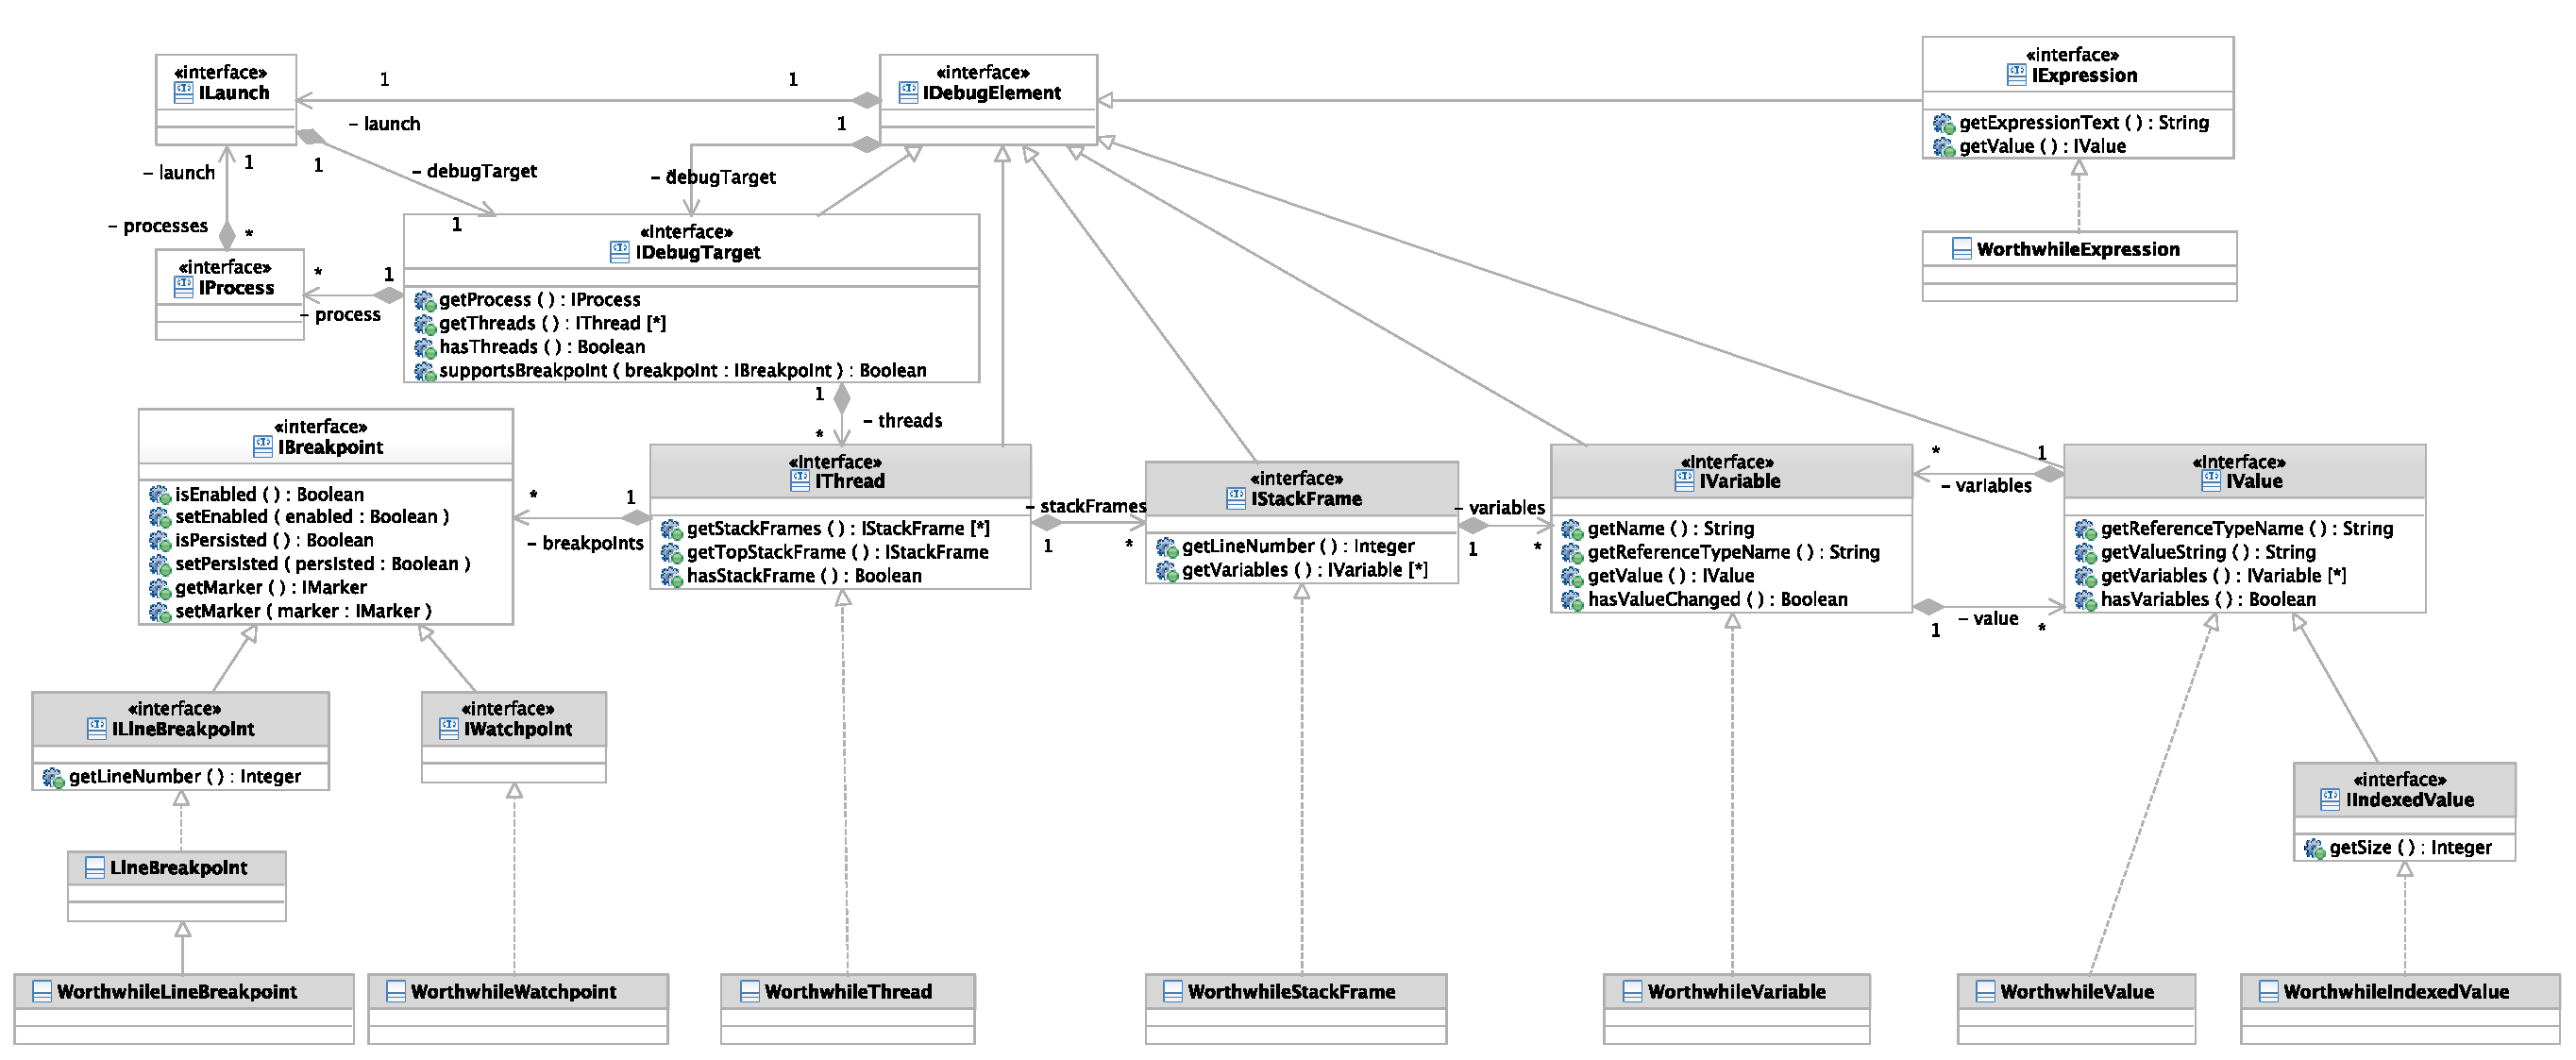
\includegraphics[angle=90,height=\textheight]{diagrams/debugmodel.pdf}
	\label{debugmodel}
\end{figure}
\footnotetext{basierend auf \url{http://www.eclipse.org/articles/Article-Debugger/how-to.html}}

\subsubsection{class WorthwhileDebugTarget}

Diese Klasse stellt die Schnittstelle zwischen GUI und Interpreter bereit. Sie übernimmt die Kommandos von der GUI und übersetzt sie in Kommandos für den Interpreter (bzw.\ dessen \texttt{DebugInterface}).

\begin{description}
	\method{public IProcess getProcess()} Gibt den Prozess zurück, der den Interpreter ausführt.
	\method{public IThread[] getThreads()} Gibt eine Liste der Threads zurück, die zu diesem Interpreterlauf gehören.
	\method{public boolean hasThreads()} Gibt an, ob momentan irgendwelche Threads vorhanden sind.
	\method{public boolean supportsBreakpoint(IBreakpoint breakpoint)} Gibt an, ob das Setzen des angegebenen Breakpoints unterstützt wird.
\end{description}

\subsubsection{class WorthwhileThread}

Ein Thread repräsentiert einen sequentiellen Programmablauf. Da die WHILE-""Sprache kein Multithreading unterstützt, gibt es für jeden Interpreterlauf nur eine Instanz dieser Klasse. Ein Thread ermöglicht den Zugriff auf \texttt{StackFrames}, wenn die Programmausführung pausiert ist.

\begin{description}
	\method{public IStackFrame[] getStackFrames()} Gibt alle in diesem Thread enthaltenen Stackframes zurück.
	\method{public IStackFrame getTopStackFrame()} Gibt den obersten Stackframe zurück.
	\method{public boolean hasStackFrame()} Gibt zurück, ob der Thread im Moment Stackframes besitzt.
\end{description}

\subsubsection{class WorthwhileStackFrame}

Ein Stackframe repräsentiert in der GUI einen Ausführungskontext eines Programms. Dazu gehören insbesondere die an der aktuellen Ausführungsposition sichtbaren Variablen.

\begin{description}
	\method{public int getLineNumber()} Gibt die Zeilennummer der Ausführungsposition in der Quelldatei zurück.
	\method{public IVariable[] getVariables()} Gibt die im Ausführungskontext sichtbaren Variablen zurück.
\end{description}

\subsubsection{class WorthwhileVariable}

Diese Klasse repräsentiert eine Variable in einem Ausführungskontext. Jede Variable besitzt einen Wert und kann verändert werden.

\begin{description}
	\method{public String getName()} Gibt den Namen der Variablen zurück.
	\method{public String getReferenceTypeName()} Gibt eine textuelle Repräsentation des Datentyps der Variablen zurück.
	\method{public IValue getValue()} Gibt den Wert der Variablen zurück.
	\method{public boolean hasValueChanged()} Gibt an, ob sich der Wert der Variablen seit der letzten Pausierung des Programmablaufs geändert hat.
\end{description}

\subsubsection{class WorthwhileValue}

Diese Klasse repräsentiert den Wert einer Variablen.

\begin{description}
	\method{public String getReferenceTypeName()} Gibt eine textuelle Repräsentation des Datentyps des Wertes zurück.
	\method{public String getValueString()} Gibt eine textuelle Repräsentation des Wertes zurück.
	\method{public IVariable[] getVariables()} Gibt eine Liste aller enthaltenen Variablen (z.~B.\ Werte in einem Array) zurück.
	\method{public boolean hasVariables()} Gibt zurück, ob dieser Wert enthaltene Variablen besitzt.
\end{description}

\subsubsection{class WorthwhileExpression}

Diese Klasse repräsentiert einen auszuwertenden benutzerdefinierten Ausdruck.

\begin{description}
	\method{public String getExpressionText()} Gibt den Quellcode des Ausdrucks zurück.
	\method{public IValue getValue()} Gibt den aktuellen Wert des Ausdrucks zurück.
\end{description}

\subsubsection{class WorthwhileLineBreakpoint}

Diese Klasse repräsentiert einen Breakpoint, der an eine bestimmte Zeile im Programmtext gebunden ist und die Programmausführung anhält, sobald diese Zeile erreicht wird.

\begin{description}
	\method{public int getLineNumber()} Gibt die Zeilennummer dieses Breakpoints zurück.
	\method{public IMarker setMarker()} Setzt die Markierung, die diesem Breakpoint zugeordnet ist. Diese Markierung enthält alle notwendigen Informationen zum Breakpoint und wird auch über das Ende einer GUI-""Sitzung hinaus gespeichert.
\end{description}

\subsubsection{class WorthwhileWatchpoint}

Diese Klasse repräsentiert einen \textit{Watchpoint}, also einen Breakpoint, der an eine Variable gebunden ist und die Programmausführung anhält, sobald ihr Wert gelesen oder verändert wird.

\begin{description}
	\method{public IMarker setMarker()} Setzt die Markierung, die diesem Breakpoint zugeordnet ist. Diese Markierung enthält alle notwendigen Informationen zum Breakpoint und wird auch über das Ende einer GUI-""Sitzung hinaus gespeichert.
\end{description}

\subsection{Launching}

\subsubsection{class WorthwhileLaunchDelegate}

Der \texttt{LaunchDelegate} ist dafür verantwortlich, den Interpreter zu starten und zu initialisieren sowie die Verbindung zwischen Interpreter und Debug-""Infrastruktur herzustellen.

\begin{description}
	\mlmethod{public void launch(ILaunchConfiguration~configuration, String~mode, ILaunch~launch, IProgressMonitor~monitor)}
	Diese Methode wird von der GUI aufgerufen, wenn der Benutzer den Befehl zum Ausführen des Programms wählt. Dabei enthält \texttt{configuration} die nötigen Einstellungen zum Aufruf des Interpreters, etwa den Pfad zur ausführbaren Datei von Z3 oder Optionen für den Interpreter. \texttt{mode} enthält den Modus, in dem das Programm ausgeführt wird, und ist entweder \texttt{run} oder \texttt{debug}. Der Parameter \texttt{launch} enthält Informationen über diese Ausführung des Programms; die Aufgabe dieser Methode ist es, sämtliche erzeugten Prozesse und \texttt{DebugTarget}s diesem Objekt bekannt zu machen. Schließlich kann der Fortschritt der Ausführung dem Benutzer über das \texttt{monitor}-""Objekt mitgeteilt werden.
\end{description}

\subsubsection{class WorthwhileSourcePathComputerDelegate}

Diese Klasse ist dafür verantwortlich, die Pfade zu bestimmen, die auf der Suche nach Quelldateien (Source Lookup) durchsucht werden sollen. Ein Source Lookup wird immer dann nötig, wenn der aktuelle Ausführungszustand des Interpreters auf die Quelldatei zurückgeführt werden soll, etwa bei der Anzeige der aktuell ausgeführten Zeile.

\begin{description}
	\mlmethod{public ISourceContainer[] computeSourceContainers( ILaunchConfiguration~configuration, IProgressMonitor~monitor)}
	Ruft eine Liste aller Pfade ab, die beim Source Lookup nach Quelldateien durchsucht werden.
\end{description}

\subsubsection{class WorthwhileSourceLookupParticipant}

Für den Source Lookup kann sich eine Reihe von Klassen (Participants) registrieren, die ein Objekt einer Quelldatei zuordnen. Ein solcher Participant wird in dieser Klasse implementiert.

\begin{description}
	\method{public String getSourceName(Object object)} Ruft den Quelldateinamen für \texttt{object} ab, wenn es sich dabei um eine Instanz von \texttt{WorthwhileStackFrame} handelt.
\end{description}

\subsubsection{class WorthwhileSourceLookupDirector}

Diese Klasse ist dafür verantwortlich, den \texttt{SourceLookupParticipant} der Debugger-""Infrastruktur bekannt zu machen.

\begin{description}
	\method{public void initializeParticipants()} Macht der Debugger-""Infrastruktur die Objekte bekannt, die am Source Lookup teilnehmen sollen.
\end{description}

\section{Abweichungen von den Ergebnissen der Planungsphase}
Die in der Entwurfsphase angestellten Überlegungen haben ergeben, dass die im Pflichenheft spezifizierten Anforderungen sinnvoll sind und größtenteils in dem gegebenen Zeitrahmen erfüllt werden können. Trotzdem wurden einige Punkte festgestellt, an denen der Aufwand für den Entwurf sowie die Spezifikation bestimmter Funktionalität falsch eingeschätzt wurde.

\subsection{Interpreter}
In der Planungsphase wurde stets von einer separaten Komponente "`Run-""time""-Checker"' ausgegangen, deren Aufgabe die Auswertung der im Programmtext eingebetteten Annotationen umfassen sollte. Im Entwurf hat sich gezeigt, dass sich die in den Annotationen angegebenen Ausdrücke sowohl syntaktisch als auch semantisch, mit dem Unterschied der nur in der Annotationssprache erlaubten quantifizierten Aussagen, nicht von denen in der WHILE-""Sprache unterscheiden. Aus diesem Grunde wurde die Entwurfsentscheidung getroffen, die Komponente "`Run-""time-""Checker"' in die Komponente "`Interpreter"' zu integrieren. Der Interpreter soll nun auch quantifizierte Ausdrücke auswerten können, bei Bedarf auch unter Zuhilfenahme der Beweiserschnittstelle.

\section{Planung der Implementierungsphase}

Die Implementierungsphase lässt sich grob in sechs Phasen (Vorbereitung, Parser, Interpreter, Beweiserschnittstelle, GUI, Dokumentation) einteilen. Die ungefähre Zeitplanung und die Abhängigkeiten jedes Arbeitsschrittes ist in Abbildung \ref{gantt_impl} verdeutlicht.

\begin{figure}
	\centering
	\hspace*{-2cm}\vspace*{-2cm}\caption[B]{Die Tasks der Implementierungsphase und ihre Abhängigkeiten}
	\hspace*{-3cm}\vspace*{-3cm}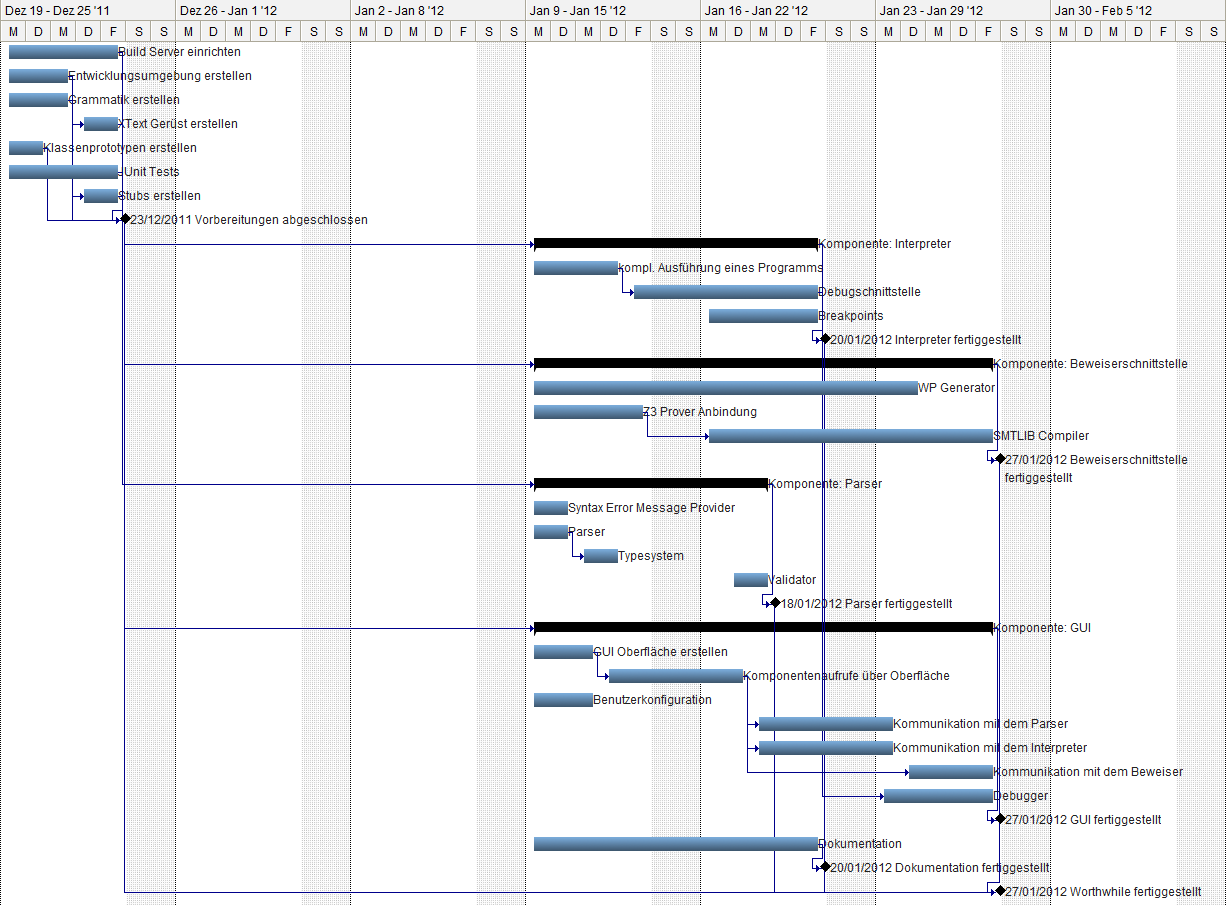
\includegraphics[angle=90,width=19cm,height= 25cm]{diagrams/gantt_implementierung_diag.png}
	
	\label{gantt_impl}
\end{figure}

\subsection{Vorbereitungen}
In der Vorbereitungsphase, welche allen anderen Phasen voranliegt, wird hauptsächlich das Klassendiagramm in Quelltext umgesetzt, sowie ein Basis für die Implementierungen eingerichtet. Hierzu gehört insbesondere das Erstellen der Grammatik für die while-Sprache und das Ausrüsten aller Komponenten mit Stubs um eingeschränkt funktionierende Schnittstellen für die anderen Teile des Programms bereit zu stellen. Desweiteren werden JUnit Tests erstellt, die implementierungsbegleitend benutzt werden sollen. Durch die vorgesehenen Stubs sollten alle JUnit Tests erfolgreich ausgführt werden können. Im späteren Verlauf der Implementierungsphase wird Wert darauf gelegt, dass ein Stub nur dann gegen eine funktionierende Schnittstelle ausgetauscht wird, wenn gewährleistet ist, dass der zuständige JUnit Test immer noch erfolgreich abläuft. Für diese Phase werden alle Mitglieder des Teams in etwa gleich beansprucht. Nach erfolgreicher Beendigung der Vorbereitungen können die Phasen für die jeweiligen Komponenten des Projekts (Interpreter mit Runtime Checker, Beweiserschnittstelle, GUI) anlaufen.

\subsection{Parser}
Möglichst frühzeitig wird die Parserfunktionalität soweit erstellt, dass das parsen eines Programms möglich ist. Dieser Teil ist von hoher Wichtigkeit, da hierdurch das übrige Projekt auf einen eigens erstellten AbstractSyntaxTree (jedoch ohne semantische Prüfung) zurückgreifen kann und nicht mehr abhängig von der Ausgabe des Stubs ist.

[TODO] Syntax Error Message Provider?

Anschließend kann die Einbindung des Typsystems erfolgen und die Funktionalität des Validators aufgenommen werden.

\subsection{Interpreter}
Zu Beginn dieser Phase erfolgt die Implementierung der Grundfunktionalität des Interpreters. Die komplette Ausführung eines ASTs soll  ermöglicht werden um Fehler des vom Parser erzeugten AbstactSyntaxTrees frühzeitig zu erkennen. Einen hohen Stellenwert bekommt die Debugschnittstelle welche direkt nach Implementierung der Grundfunktionalität entwickelt wird. Die Einbindung der Unterstützung für Breakpoints kann parallel hierzu erfolgen.

\subsection{Beweiserschnittstelle}
In dieser Phase ist der Teil für die Generierung der Weakest Precondition Formel größtenteils unabhängig von der Anbindung des Beweiser und des Compilers für die SMTLIB Sprache und kann somit parallel hierzu bearbeitet werden. Die Umwandlung in SMTLIB Sprache ist abhängig von der Anbindung des Beweisers, da es hiermit ermöglicht wird, seinen SMTLIB Compiler zu testen und damit auch korrekt zu implementieren.

\subsection{GUI}
Die GUI kann in vielen Bereichen unabhängig vom Rest des Projekts entwickelt werden. Es ist jedoch von Vorteil die Kommunikation mit den einzelnen Komponenten erst dann zu implementieren wenn eine gewisse Grundfunktionalität der jeweiligen Komponente gegeben ist. Deshalb wird die Oberfläche der GUI zu Beginn erstellt und anschließend die Aufrufe von der Oberfläche zu den Kommunikationsschnittstellen integriert. Gleichzeitig kann mit der Implementierung des Teils der Benutzerkonfiguration erfolgen. Erst dann wird mit der Implementierung der Kommunikationskomponenten begonnen. Der Debugger wird entwickelt sobald der Interpreter fertiggestellt ist.

\subsection{Dokumentation}
Die Dokumentation wird begleitend mit allen Phasen erstellt und sichert Konsistenz und Vollständigkeit. Desweiteren ist es hilfreich diese eher zu Beginn zu entwickeln, da dies wiederum die Implementierung unterstützt. Bei dieser Phase wird jedes Teammitglied, überwiegend in seinem zugehörigen Bereich, beteiligt sein.


\clearpage
\appendix

\end{document}
